
\documentclass[a4paper,12pt, fleqn]{article}
% fleqn - Выравнивание формул по левому краю


%%% Работа с русским языком
\usepackage{cmap}					% поиск в PDF
\usepackage{mathtext} 				% русские буквы в формулах
\usepackage[T2A]{fontenc}			% кодировка
\usepackage[utf8]{inputenc}			% кодировка исходного текста
\usepackage[english,russian]{babel}	% локализация и переносы
\usepackage{setspace}
% одинарный интервал
\singlespacing
\small
\renewcommand{\labelenumii}{\arabic{enumi}.\arabic{enumii}.}
\renewcommand{\labelenumiii}{\arabic{enumi}.\arabic{enumii}.\arabic{enumiii}.}


%%% Дополнительная работа с математикой
\usepackage{amsmath,amsfonts,amssymb,amsthm,mathtools} % AMS
\usepackage{icomma} % "Умная" запятая: $0,2$ --- число, $0, 2$ --- перечисление

%%% Работа с цветом
\usepackage[usenames]{color}
\usepackage{colortbl}

%% Номера формул
%\mathtoolsset{showonlyrefs=true} % Показывать номера только у тех формул, на которые есть \eqref{} в тексте.
%\usepackage{leqno} % Нумерация формул слева

%% Свои команды
\DeclareMathOperator{\sgn}{\mathop{sgn}}

%% Перенос знаков в формулах (по Львовскому)
\newcommand*{\hm}[1]{#1\nobreak\discretionary{}
	{\hbox{$\mathsurround=0pt #1$}}{}}

%%% Работа с картинками
\usepackage{graphicx}  % Для вставки рисунков
\graphicspath{{images/}{WinLogic/}}  % папки с картинками
\setlength\fboxsep{3pt} % Отступ рамки \fbox{} от рисунка
\setlength\fboxrule{1pt} % Толщина линий рамки \fbox{}
\usepackage{wrapfig} % Обтекание рисунков текстом

%%% Работа с таблицами
\usepackage{array,tabularx,tabulary,booktabs} % Дополнительная работа с таблицами
\usepackage{longtable}  % Длинные таблицы
\usepackage{multirow} % Слияние строк в таблице

%%% Теоремы
\theoremstyle{plain} % Это стиль по умолчанию, его можно не переопределять.
%\newtheorem{theorem}{Теорема}[section]
%\newtheorem{proposition}[theorem]{Утверждение}

\theoremstyle{definition} % "Определение"
%\newtheorem{corollary}{Следствие}[theorem]
%\newtheorem{problem}{Задача}[section]

\theoremstyle{remark} % "Примечание"
\newtheorem*{nonum}{Решение}

%%% Программирование
\usepackage{etoolbox} % логические операторы


%%% Функции, свяханные с этим документом
\newcommand{\DocumentNum}{
	RU.17701729.506900-01 ТЗ 01-1
}

\newcommand{\Changing}{
	\ensuremath{
		$$
		\begin{array}{|c|c|c|c|c|}
		\hline
		&&&&\\
		\hline
		\text{Изм.}&\text{Лист}&\text{№ докум.}&\text{Подп.}&\text{Дата}\\
		\hline
		\text{\DocumentNum}&&&&\\
		\hline
		\text{Инв. № подл.}&\text{Подп. и дата}&\text{Взам. инв. №}&\text{Инв. № дубл.}&\text{Подп. и дата}\\
		\hline
		\end{array}
		$$
	}
}


%%% Страница
%\usepackage{extsizes} % Возможность сделать 14-й шрифт
\usepackage{geometry} % Простой способ задавать поля
\geometry{top=20mm}
\geometry{bottom=20mm}
\geometry{left=30mm}
\geometry{right=10mm}
%
\usepackage{fancyhdr} % Колонтитулы
\pagestyle{fancy}
\renewcommand{\headrulewidth}{0mm}  % Толщина линейки, отчеркивающей верхний колонтитул
\lfoot{}%Нижний левый
\rfoot{}%Нижний правый
\rhead{Вариант 12}%Верхний правый
\chead{Торилов Дмитрий}%Верхний в центре
\lhead{}%Верхний левый
\cfoot{\thepage} % По умолчанию здесь номер страницы


\usepackage{setspace} % Интерлиньяж
\onehalfspacing % Интерлиньяж 1.5
%\doublespacing % Интерлиньяж 2
%\singlespacing % Интерлиньяж 1

\usepackage{lastpage} % Узнать, сколько всего страниц в документе.

\usepackage{soulutf8} % Модификаторы начертания

\usepackage{hyperref}
\usepackage[usenames,dvipsnames,svgnames,table,rgb]{xcolor}
\definecolor{my-color}{HTML}{000000}
\hypersetup{				% Гиперссылки
	unicode=true,           % русские буквы в раздела PDF
	pdftitle={Пояснительная записка},   % Заголовок
	pdfauthor={Автор},      % Автор
	pdfsubject={КДЗ по программированию},      % Тема
	pdfcreator={Создатель}, % Создатель
	pdfproducer={Производитель}, % Производитель
	pdfkeywords={keyword1} {key2} {key3}, % Ключевые слова
	colorlinks=true,       	% false: ссылки в рамках; true: цветные ссылки
	linkcolor=black,          % внутренние ссылки
	citecolor=black,        % на библиографию
	filecolor=magenta,      % на файлы
	urlcolor=black           % на URL
}

%\renewcommand{\familydefault}{\sfdefault} % Начертание шрифта

\usepackage{csquotes} % Инструменты для ссылок

%\usepackage[bibencoding=utf8]{biblatex}
%\addbibresource{bib1.bib}
%\addbibresource{GOST.bib}

% Обещают Times New Roman
%\renewcommand{\rmdefault}{ftm}


\usepackage{multicol} % Несколько колонок

\author{Торилов Дмитрий}
\title{Пояснительная записка}
\date{\today}


%\textbf{полужирный шрифт}
%\textit{курсивом}

\newcommand{\mc}[1]{%
	%\underline{#1}%\colorbox{YellowGreen}{#1}%
	%\ensuremath{
	%	{\textcolor{blue}{\textbf{#1}}}
	%}
	%\boldsymbol{#1}
	\cellcolor{YellowGreen}#1
} % blue color highlighting
%\textcolor{blue}{\textbf{Синий}}

%%% Нумeрация формул зависит от раздела
\numberwithin{equation}{section}


%%% Программирование на LaTeX
\usepackage{forloop}


\newcommand{\Ssign}{\underline{\hspace{8em}}}


\newcommand{\PeopleField}[1]{
	\vbox to 10em{
		#1\\
		<<\underline{\hspace{1.8em}}>>
		\underline{\hspace{10.5em}}
		2018 г.
	}
}


\newcommand{\StorageTable}{
	$$
	\begin{tabular}{|m{5mm}|p{7mm}|}
	\hline
	\rotatebox{90}{
		Дата и подп.
	}&\rule{0mm}{35mm}\\
	\hline
	\rotatebox{90}{
		Инв. № дубл.
	}&\rule{0mm}{25mm}\\
	\hline
	\rotatebox{90}{
		Взвм. инв. №
	}&\rule{0mm}{25mm}\\
	\hline
	\rotatebox{90}{
		Дата и подп.
	}&\rule{0mm}{35mm}\\
	\hline
	\rotatebox{90}{
		Инв. № подл.
	}&\rule{0mm}{25mm}\\
	\hline
	\end{tabular}
	$$
}

%%% Содержание
\renewcommand{\thesection}{\arabic{section}.}
\renewcommand{\thesubsection}{\arabic{section}.\arabic{subsection}.}
\renewcommand{\thesubsubsection}{\arabic{section}.\arabic{subsection}.\arabic{subsubsection}.}
\makeatletter
\renewcommand{\l@section}{\@dottedtocline{1}{0.5em}{1.5em}}
\renewcommand{\l@subsection}{\@dottedtocline{1}{1.5em}{2.5em}}
\renewcommand{\l@subsubsection}{\@dottedtocline{1}{3em}{3em}}
\makeatother

\usepackage{listings}

\begin{document}

\begin{titlepage}
		
	\large
	\begin{center}
		НАЦИОНАЛЬНЫЙ ИССЛЕДОВАТЕЛЬСКИЙ УНИВЕРСИТЕТ\\
		<<ВЫСШАЯ ШКОЛА ЭКОНОМИКИ>>\\
		Дисциплина: <<Программирование>>\\[10em]
		
		Контрольное домашнее задание\\
		3 модуль\\
		Вариант 12\\[7em]	
	\end{center}
	
	\begin{flushright}
		\PeopleField{
			Выполнил\\
			Студент группы БПИ173\\
			\Ssign /Д. М. Торилов/
		}
		
		Преподаватель: Максименкова О.В.,\\
		старший преподаватель\\
		департамента\\
		программной инженерии\\
		факультета компьютерных наук\\[7em]
	\end{flushright}
	
	\begin{center}
		Москва 2017	
	\end{center}
	
	\normalsize
	\newpage

\end{titlepage}

% Оглавление
\setcounter{page}{2}
\tableofcontents
\newpage

\section{Условие задачи}
Программа контрольного домашнего задания (КДЗ) должна представлять собой небольшую информационно-справочную систему (ИСС), основанную на файлах. В стандартном файле содержатся данные о землетрясениях. Данные из него загружаются в основную таблицу ИСС.\\[1em]
Далее следует описание задания варианта \textnumero 12:\\[1em]
Для представления данных о землетрясении использовать класс EarthQuake. Координаты землетрясения представлять объектом структуры. Класс QuakeInfo связан с объектами EarthQuake отношением агрегации и позволяет получать списки землетрясений, сгруппированные по количеству уловивших их станций; списки землетрясений с максимальной магнитурой; землетрясение произошедшее на минимальной и максимальной глубине. Модифицировать интерфейс так, чтобы указанные данные можно было отобразить.\\


\section{Функции разрабатываемого приложения}

\subsection{Варианты использования}
Данная ИСС может быть использована для проведения исследований в области изучения землетрясений, в том числе в научных и образовательных целях.

\subsection{Описание интерфейса пользователя}
Интерфейс программы реализован на русском языке. В реализации использована технология Windows Forms. В дальнейшем будет совершён переход на технологию WPF.\\
Интерфейс программы включает в себя:
\subsubsection{Панель меню}
\begin{enumerate}
	\item Кнопка \textbf{Файл}, даёт доступ к кнопкам:
	\begin{enumerate}
		\item Кнопка \textbf{Открыть}, позволяет вызвать меню выбора файла для открытия
		\item Кнопка \textbf{Сохранить}, позволяет вызвать меню выбора файла для сохранения, либо сохранить в уже открытый файл, даёт доступ к кнопкам:
		\begin{enumerate}
			\item \textbf{Дозаписать}, позволяет вызвать меню выбора файла для дозаписи таблицы в его конец, либо сохранить в уже открытый файл
		\end{enumerate}
		\item Кнопка \textbf{Сохранить как}, позволяет вызвать меню выбора файла для сохранения, даёт доступ к кнопкам:
		\begin{enumerate}
			\item \textbf{Дозаписать}, позволяет вызвать меню выбора файла для дозаписи таблицы в его конец
		\end{enumerate}
		\item \textbf{Закрыть}, позволяет прекратить работу с файлом, вызывает диалоговое окно с предложением сохранить файл перед закрытием				
	\end{enumerate}
	\item Кнопка \textbf{Таблица}, даёт доступ к кнопкам:
	\begin{enumerate}
		\item Кнопка \textbf{Сортировка}, даёт доступ к кнопкам:
		\begin{enumerate}
			\item \textbf{По номеру}, позволяет отсортировать таблицу по возрастанию идентификационных номеров элементов
			\item \textbf{По станциям}, позволяет отсортировать таблицу по вохрастанию числа в количественной характеристике станций, засёкших землетрясение, соответствующее элементу			
		\end{enumerate}
		\item Кнопка \textbf{Удалить выделенную строку}, позволяет удалить выделенную строку из таблицы				
	\end{enumerate}
	\item Кнопка \textbf{Информация}, даёт доступ к кнопкам:
	\begin{enumerate}
		\item \textbf{Предельные значения}, позволяет увидеть короткий список диапазонов изменения характеристических величин элементов таблицы
		\item \textbf{О программе}, позволяет увидеть информацию об авторе программы
	\end{enumerate}
\end{enumerate}
\subsubsection{Панель управления}
\begin{enumerate}
	\item Поле \textbf{Добавление элемента} включает в себя
	\begin{enumerate}
		\item Поле ввода \textbf{Номер элемента}
		\item Поле ввода \textbf{Широта элемента}
		\item Поле ввода \textbf{Долгота элемента}
		\item Поле ввода \textbf{Глубина элемента}
		\item Поле ввода \textbf{Магнитуда элемента}
		\item Поле ввода \textbf{Станции элемента}
		\item Кнопка \textbf{Добавить}, создаёт элемент с характеристиками 1.1 - 1.6 и добавляет его в таблицу		
	\end{enumerate}	
	\item Поле \textbf{Землетрясения} включает в себя два подполя, \textbf{Максимальная глубина} (информация о землетрясении с максимальной глубиной) и \textbf{Минимальная глубина} (информация о землетрясении с минимальной глубиной), несущие полную информацию о таковых в таблице в режиме реального времени
	\item Поле \textbf{Фильтрация по магнитуде} включает в себя два
	\begin{enumerate}
		\item Поле ввода \textbf{Магнитуда} для ввода вещественного значения магнитуды  
		\item Кнопка \textbf{Фильтровать}, при нажатии удаляет из таблицы все данные о землетрясениях, магнитудой ниже чем в поле 3.1
	\end{enumerate}
	\item Кнопка \textbf{Выход} позволяет выйти из приложения
\end{enumerate}
\subsubsection{Панель работы с таблицей}
Представляет из себя матрицу неограниченного числа строк и 6 столбцов с возможностью редактирования  
\subsubsection{Всплывающие подсказки}
Появляются при наведении курсора мыши на необходимый элемент. Несут дополнительную информацию об объекте.

\section{Структура приложения}
Приложение реализовано с использованием паттерна Model-View-Controller\cite{MVC}. Model реализована объектом класса QuakeInfo. View реализована объектом Form1. Задачу Controller выполняет статический класс Jarvis. Ниже приведены необходимые для понимания детали структуры приложения.
\subsection{Диаграмма классов}
\newpage
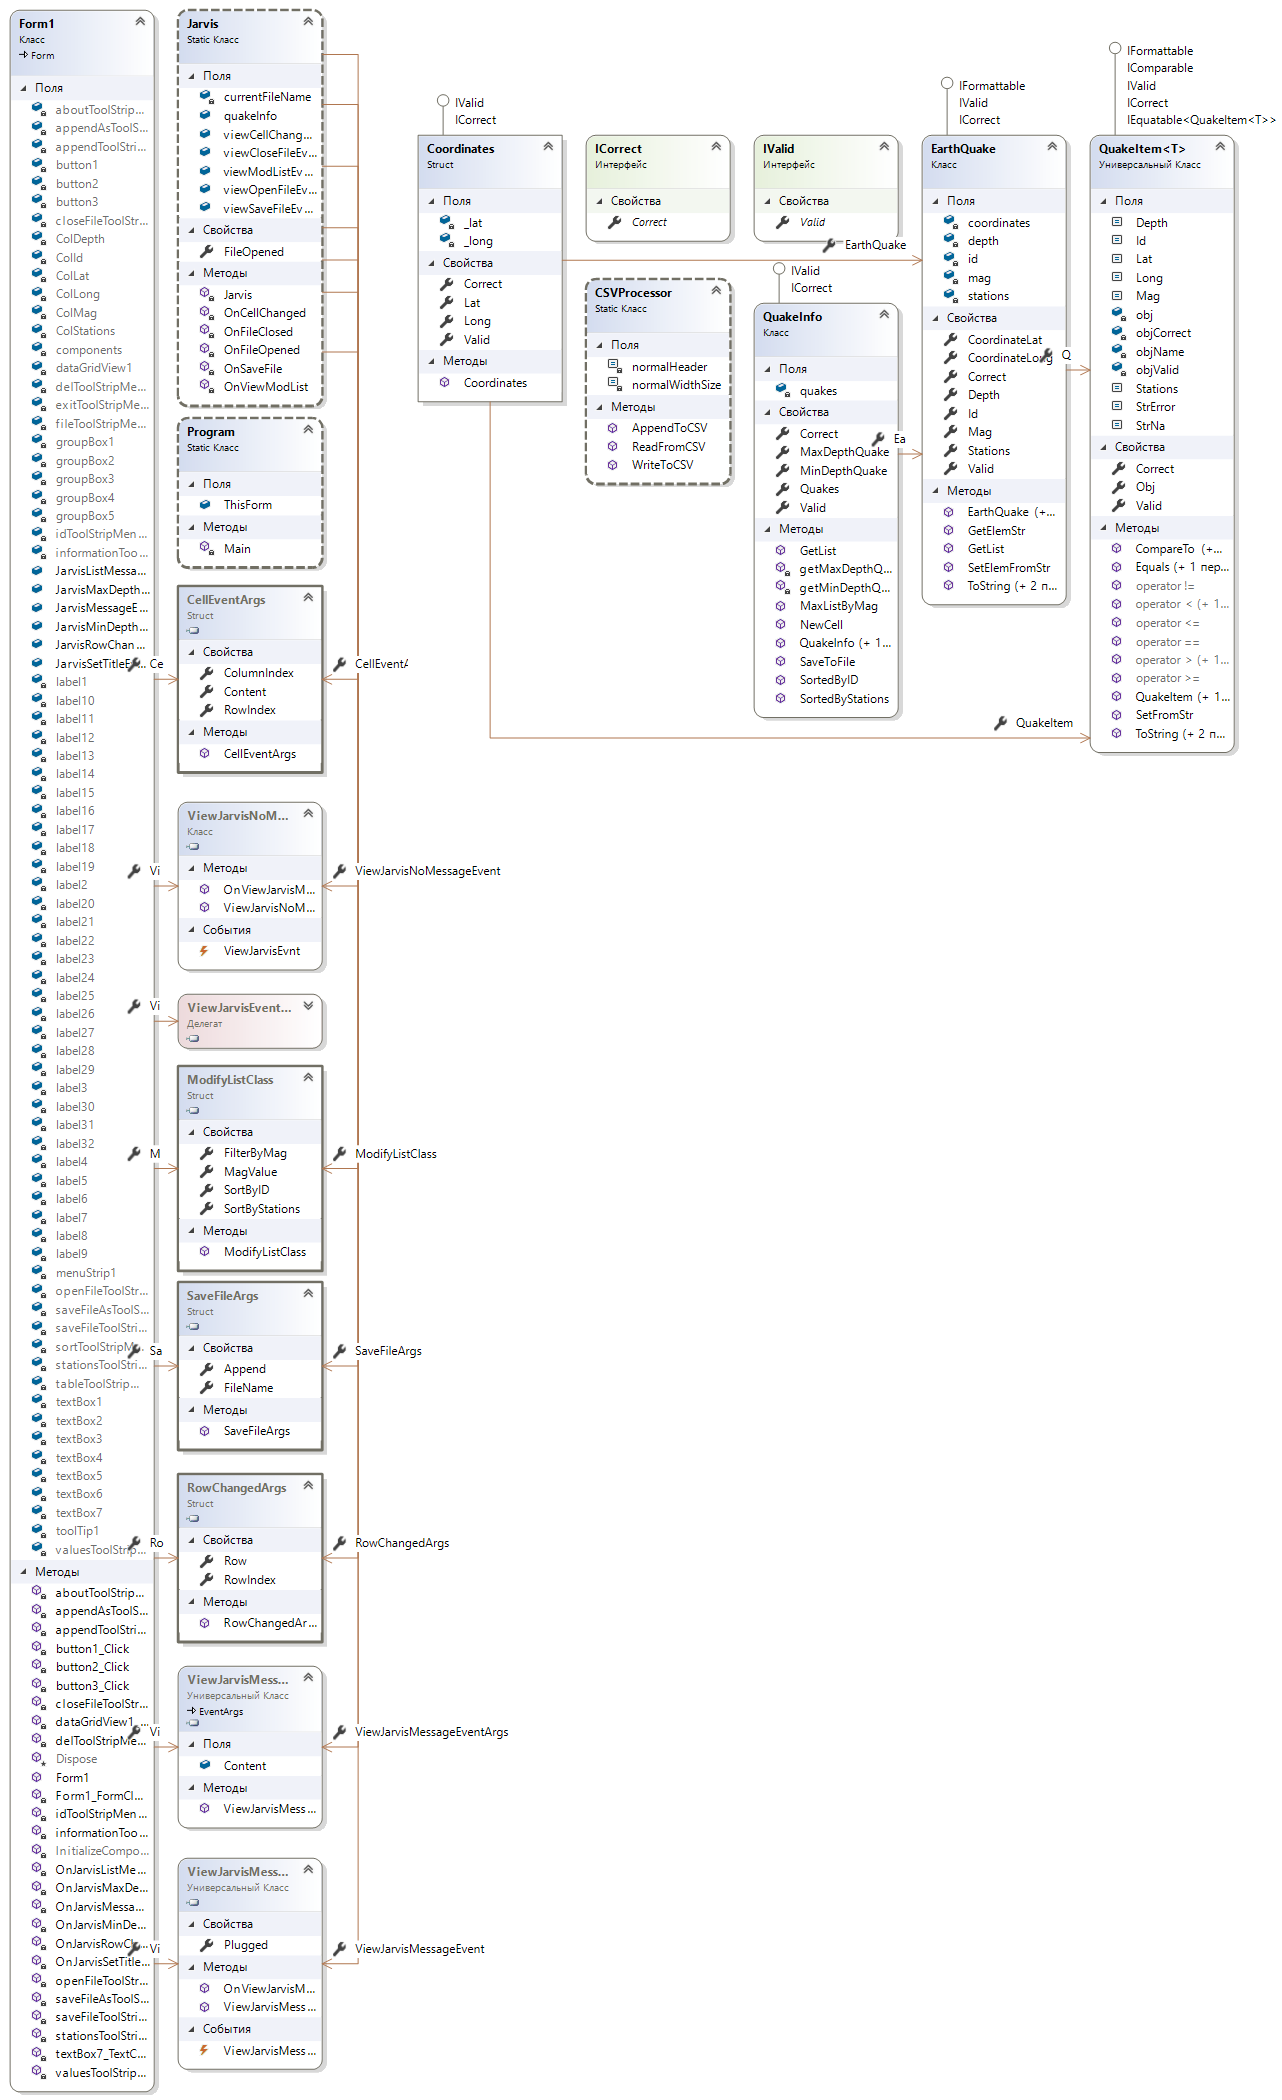
\includegraphics[width=1\linewidth]{ClassDiagram4.png}
\subsection{Описание классов, их полей и методов}

\subsubsection{Jarvis}
Выполняет задачу синхронизации Model и View.\\
Объект класса QuakeInfo связан со статическим классом Jarvis отношением агрегации.\\
С объектом Form1 реализовано гибкое общение через события\cite{Ev} с обобщениями\cite{Gen}\cite{Ev2}.\\[2em]
\textbf{Поля}:
\begin{itemize}
	\item public static QuakeInfo quakeInfo - Модель агрегирована в контроллер
	\item private static string currentFileName = null; - Имя файла, с которым ведётся работа
\end{itemize}


\textbf{Свойства}:

\begin{itemize}
	\item public static bool FileOpened => currentFileName != null; - Свойство корректного открытия файла
\end{itemize}

\textbf{Методы}:
\begin{itemize}
	\item private static void OnViewModList(object sender, ViewJarvisMessageEventArgs\\<ModifyListClass> messageEventArgs) - Обработчик вызова модификатора списка (сортировки и фильтрации)
	\item private static void OnFileOpened(object sender, ViewJarvisMessageEventArgs<string> messageEventArgs) - Обработчик открытия файла
	\item private static void OnSaveFile(object sender, ViewJarvisMessageEventArgs<SaveFileArgs> messageEventArgs) - Обработчик сохранения файла
	\item private static void OnFileClosed() - Обработчик закрытия файла
	\item private static void OnCellChanged(object sender, ViewJarvisMessageEventArgs\\<CellEventArgs> messageEventArgs) - Обработчик изменения ячейки
	\item static Jarvis() - Конструктор
\end{itemize}

\textbf{События}:
\begin{itemize}
	\item public static ViewJarvisMessageEvent<string> viewOpenFileEvent = new\\ ViewJarvisMessageEvent<string>(); - Событие обработчика открытия файла
	\item public static ViewJarvisMessageEvent<SaveFileArgs> viewSaveFileEvent = new\\ ViewJarvisMessageEvent<SaveFileArgs>(); - Событие обработчика сохранения файла
	\item public static ViewJarvisNoMessageEvent viewCloseFileEvent = new\\ ViewJarvisNoMessageEvent(); - Событие закрытия файла
	\item public static ViewJarvisMessageEvent<CellEventArgs> viewCellChangedEvent = new\\ ViewJarvisMessageEvent<CellEventArgs>(); - Событие обработчика изменения ячейки таблицы
	\item public static ViewJarvisMessageEvent<ModifyListClass> viewModListEvent = new\\ ViewJarvisMessageEvent<ModifyListClass>(); - Событие обработчика модификации списка
\end{itemize}
\subsubsection{Form}
Представляет реализацию View\cite{Tit}\cite{DataGridView}. Обменивается данными с Jarvis через события. 

\textbf{Методы}:
\begin{itemize}
\item private void OnJarvisMessageEvent(object sender, ViewJarvisMessageEventArgs<string> messageEventArgs) - Обработчик осбытия получения сообщения от класса Jarvis
\item private void OnJarvisListMessageEvent(object sender, ViewJarvisMessageEventArgs\\<List<List<string>>> messageEventArgs) - Обработчик события получения таблицы от класса Jarvis
\item private void OnJarvisSetTitleEvent(object sender, ViewJarvisMessageEventArgs<string> messageEventArgs) - Обработчик события вывода сообщения
\item private void OnJarvisRowChangedEvent(object sender, ViewJarvisMessageEventArgs\\<RowChangedArgs> messageEventArgs) - Обработчик события изменения строки
\item private void OnJarvisMaxDepthUpdatedEvent(object sender, ViewJarvisMessageEventArgs\\<List<string>> messageEventArgs) - Обработчик обновления информации об элементе с самой большой характеристикой глубины
\item private void OnJarvisMinDepthUpdatedEvent(object sender, ViewJarvisMessageEventArgs\\<List<string>> messageEventArgs) - Обработчик события обновления информации об элементе с минимальной характеристикой глубины
\item public Form1() - Конструктор View
\item private void openFileToolStripMenuItemClick(object sender, EventArgs e) - Обработчик нажатия кнопки открытия файла
\item private void closeFileToolStripMenuItemClick(object sender, EventArgs e) - Обработчик нажатия кнопки закрытия файла
\item private void dataGridView1CellValueChanged(object sender, DataGridViewCellEventArgs e) - Обработчик изменения ячейки таблицы
\item private void aboutToolStripMenuItemClick(object sender, EventArgs e) - Справка
\item  private void valuesToolStripMenuItemClick(object sender, EventArgs e) - Предельные величины
\item private void button1 Click(object sender, EventArgs e) - Кнопка выхода - обработчик
\item private void button2 Click(object sender, EventArgs e) - Обработчик нажатия кнопки добавления строки
\item private void Form1 FormClosing1(object sender, FormClosingEventArgs e) - Обработчик закрытия формы
\item private void idToolStripMenuItemClick(object sender, EventArgs e) - Обработчик вызова сортировки по ID
\item private void stationsToolStripMenuItemClick(object sender, EventArgs e) - Обработчик вызова сортировки по станциям
\item private void button3 Click(object sender, EventArgs e) - Обработчик нажатия кнопки фильтрации
\item private void delToolStripMenuItemClick(object sender, EventArgs e) - Обработчик нажатия кнопки удаления строки в таблице
\item private void appendToolStripMenuItemClick(object sender, EventArgs e) - Обработчик нажатия кнопки дозаписи в файл
\item private void appendAsToolStripMenuItem1Click(object sender, EventArgs e) - Обработчик нажатия кнопки дозаписи в файл
\item private void saveFileAsToolStripMenuItemClick(object sender, EventArgs e) - Обработчик нажатия кнопки сохранения файла
\item private void saveFileToolStripMenuItemClick(object sender, EventArgs e) - Обработчик нажатия кнопки сохранения файла
\end{itemize}

\textbf{События}:
\begin{itemize}
	\item public static ViewJarvisMessageEvent<string> JarvisMessageEvent = new\\ ViewJarvisMessageEvent<string>(); - Событие получения сообщения от класса Jarvis
	\item public static ViewJarvisMessageEvent<List<List<string>>> JarvisListMessageEvent = new ViewJarvisMessageEvent<List<List<string>>>(); - Событие получения таблицы от класса Jarvis
	\item public static ViewJarvisMessageEvent<string> JarvisSetTitleEvent = new\\ ViewJarvisMessageEvent<string>(); - Событие вывода сообщения
	\item public static ViewJarvisMessageEvent<RowChangedArgs> JarvisRowChangedEvent = new ViewJarvisMessageEvent<RowChangedArgs>(); - Событие изменения строки
	\item public static ViewJarvisMessageEvent<List<string>> JarvisMaxDepthUpdatedEvent = new ViewJarvisMessageEvent<List<string>>(); - Событие обновления информации об элементе с самой большой характеристикой глубины
	\item public static ViewJarvisMessageEvent<List<string>> JarvisMinDepthUpdatedEvent = new ViewJarvisMessageEvent<List<string>>(); - Событие обновления информации об элементе с минимальной характеристикой глубины
\end{itemize}

\subsection{QuakeInfo}
Описывает модель. Агрегирована в контроллер.\\
Выполняет файловый ввод-вывод\cite{StreamReader}\cite{FileDialog}, проверяет корректность введённых координат\cite{Coord},\\ глубин\cite{EartQ}, магнитуд\cite{Mag}.

\textbf{Поля}
\begin{itemize}
	\item private List<EarthQuake> quakes = new List<EarthQuake>(); - Список землетрясений
\end{itemize}

\textbf{Свойства}
\begin{itemize}
	\item public List<EarthQuake> Quakes - Свойство списка землетрясений
	\item public bool Valid - Реализация интерфейса IValid
	\item public bool Correct - Реализация интерфейса ICorrect
	\item public List<string> MinDepthQuake => getMinDepthQuake().GetList(); - Информация о землетрясении на минимальной глубине. При добавлении элемента происходит полная проверка всего списка. Требует уменьшения сложности алгоритма. Реализована за линейную сложность из-за сжатых сроков сдачи КДЗ.
	\item public List<string> MaxDepthQuake => getMaxDepthQuake().GetList(); - Информация о землетрясении на максимальной глубине. При добавлении элемента происходит полная проверка всего списка. Требует уменьшения сложности алгоритма. Реализована за линейную сложность из-за сжатых сроков сдачи КДЗ.
\end{itemize}

\textbf{Методы}
\begin{itemize}
	\item public QuakeInfo() - Конструктор объекта
	\item public QuakeInfo(string filename) - Конструктор объекта с чтением списка из файла
	\item public List<EarthQuake> SortedByID() - Возвращает отсортированный по id список землетрясений
	\item public List<EarthQuake> SortedByStations() - Возвращает отсортированный по количеству станций список землетрясений
	\item public List<EarthQuake> MaxListByMag(double minValue) - Возвращает отсортированный по магнитуре список максимальных землетрясений
	\item private EarthQuake getMinDepthQuake() - Поиск землетрясения, произошеднего на минимальной глубине.
	\item private EarthQuake getMaxDepthQuake() - Поиск землетрясения, произошеднего на максимальной глубине.
	\item public List<List<string>> GetList(CultureInfo cultureInfo=null) - Получить представление в виде списка списков строк
	\item public List<string> NewCell(string val, int columnIndex, int rowIndex, CultureInfo\\ cultureInfo) - Установка нового значения ячейки и возвращение нового списка строк строки таблицы
	\item public void SaveToFile(string filename, string mode) - Запись и дозапись списка в файл 
\end{itemize}

\section{Распределение исходного кода по файлам проекта}
Описание модели содержится в файле QuakeInfo.cs. Все файлы из библиотеки классов ModelLibrary являются вспомогательными.\\
Описание контроллера содержится в файле Jarvis.cs.\\
Работа с интерфейсом описана в Form1.cs.
События для обмена информацией между Jarvis и Form1 описаны в библиотеке классов EventsLibrary.


\section{Контрольный пример и описание результатов}
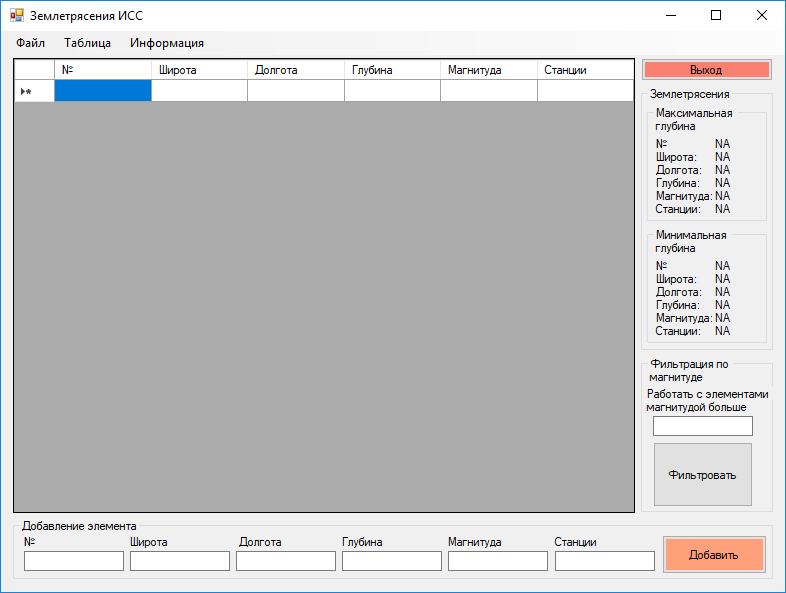
\includegraphics[width=1\linewidth]{q1.png}


\section{Текст (код) программы}
\subsection{Events Library}
\subsubsection{ViewJarvisMessage}
%\lstinputlisting{ViewJarvisMessage.cs}
%\subsection{KDZ}
%\subsubsection{Form1}
%\lstinputlisting{Form1.cs}
%\subsubsection{Jarvis}
%\lstinputlisting{Jarvis.cs}
%\subsection{ModelLibrary}
%\subsubsection{QuakeInfo}
%\lstinputlisting{QuakeInfo.cs}
%\subsubsection{CSVProcessor}
%\lstinputlisting{CSVProcessor.cs}

\newpage

\section{Список литературы}

\bibliographystyle{plain}
\bibliography{bibfile}

\end{document}